% Generated by tools/ca_figures.py from seed 11, flower 0. Do not edit.
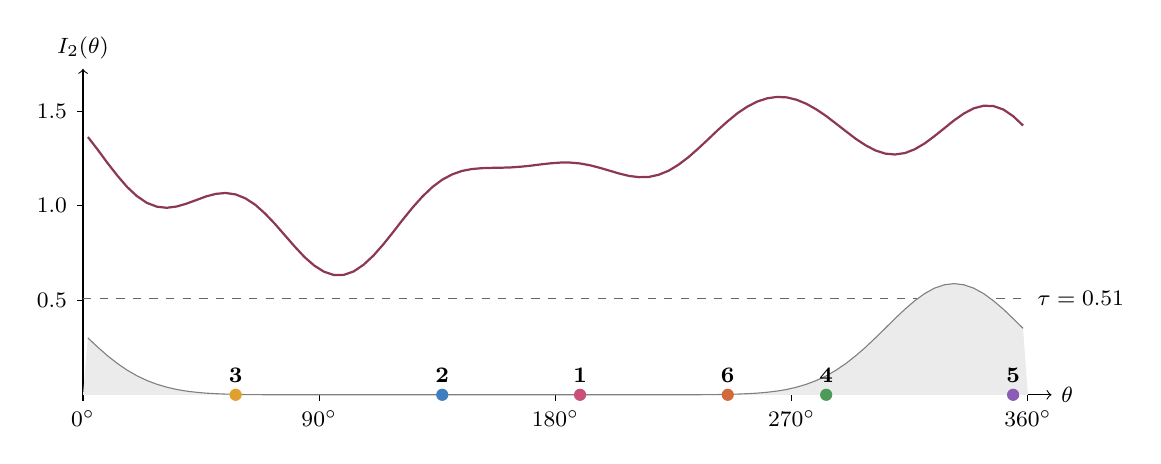
\begin{tikzpicture}[font=\footnotesize]
\definecolor{petA}{HTML}{C8507A}\definecolor{petB}{HTML}{3F7FBF}
\definecolor{petC}{HTML}{E0A030}\definecolor{petD}{HTML}{4E9A5B}
\definecolor{petE}{HTML}{8A5CB8}\definecolor{petF}{HTML}{D2693C}
\definecolor{petG}{HTML}{3AA6A0}\definecolor{petH}{HTML}{8C8C3A}
\draw[->] (0,0) -- (12.30,0) node[right] {$\theta$};
\draw[->] (0,0) -- (0,4.14) node[above] {$I_2(\theta)$};
\draw (0.000,0) -- (0.000,-0.08) node[below] {$0^\circ$};
\draw (3.000,0) -- (3.000,-0.08) node[below] {$90^\circ$};
\draw (6.000,0) -- (6.000,-0.08) node[below] {$180^\circ$};
\draw (9.000,0) -- (9.000,-0.08) node[below] {$270^\circ$};
\draw (12.000,0) -- (12.000,-0.08) node[below] {$360^\circ$};
\draw (0,1.200) -- (-0.08,1.200) node[left] {0.5};
\draw (0,2.400) -- (-0.08,2.400) node[left] {1.0};
\draw (0,3.600) -- (-0.08,3.600) node[left] {1.5};
\draw[black!60, dashed] (0,1.221) -- (12.000,1.221) node[right, black] {$\tau=0.51$};
\fill[black!8] plot coordinates {(0.062,0.722) (0.188,0.604) (0.312,0.495) (0.438,0.397) (0.562,0.312) (0.688,0.240) (0.812,0.181) (0.938,0.134) (1.062,0.097) (1.188,0.068) (1.312,0.047) (1.438,0.032) (1.562,0.021) (1.688,0.014) (1.812,0.009) (1.938,0.006) (2.062,0.003) (2.188,0.002) (2.312,0.001) (2.438,0.001) (2.562,0.000) (2.688,0.000) (2.812,0.000) (2.938,0.000) (3.062,0.000) (3.188,0.000) (3.312,0.000) (3.438,0.000) (3.562,0.000) (3.688,0.000) (3.812,0.000) (3.938,0.000) (4.062,0.000) (4.188,0.000) (4.312,0.000) (4.438,0.000) (4.562,0.000) (4.688,0.000) (4.812,0.000) (4.938,0.000) (5.062,0.000) (5.188,0.000) (5.312,0.000) (5.438,0.000) (5.562,0.000) (5.688,0.000) (5.812,0.000) (5.938,0.000) (6.062,0.000) (6.188,0.000) (6.312,0.000) (6.438,0.000) (6.562,0.000) (6.688,0.000) (6.812,0.000) (6.938,0.000) (7.062,0.000) (7.188,0.000) (7.312,0.000) (7.438,0.000) (7.562,0.000) (7.688,0.001) (7.812,0.001) (7.938,0.002) (8.062,0.003) (8.188,0.006) (8.312,0.009) (8.438,0.014) (8.562,0.021) (8.688,0.032) (8.812,0.047) (8.938,0.068) (9.062,0.097) (9.188,0.134) (9.312,0.181) (9.438,0.240) (9.562,0.312) (9.688,0.397) (9.812,0.495) (9.938,0.604) (10.062,0.722) (10.188,0.845) (10.312,0.968) (10.438,1.087) (10.562,1.194) (10.688,1.285) (10.812,1.354) (10.938,1.397) (11.062,1.412) (11.188,1.397) (11.312,1.354) (11.438,1.285) (11.562,1.194) (11.688,1.087) (11.812,0.968) (11.938,0.845)} -- (12.000,0) -- (0,0) -- cycle;
\draw[black!50] plot coordinates {(0.062,0.722) (0.188,0.604) (0.312,0.495) (0.438,0.397) (0.562,0.312) (0.688,0.240) (0.812,0.181) (0.938,0.134) (1.062,0.097) (1.188,0.068) (1.312,0.047) (1.438,0.032) (1.562,0.021) (1.688,0.014) (1.812,0.009) (1.938,0.006) (2.062,0.003) (2.188,0.002) (2.312,0.001) (2.438,0.001) (2.562,0.000) (2.688,0.000) (2.812,0.000) (2.938,0.000) (3.062,0.000) (3.188,0.000) (3.312,0.000) (3.438,0.000) (3.562,0.000) (3.688,0.000) (3.812,0.000) (3.938,0.000) (4.062,0.000) (4.188,0.000) (4.312,0.000) (4.438,0.000) (4.562,0.000) (4.688,0.000) (4.812,0.000) (4.938,0.000) (5.062,0.000) (5.188,0.000) (5.312,0.000) (5.438,0.000) (5.562,0.000) (5.688,0.000) (5.812,0.000) (5.938,0.000) (6.062,0.000) (6.188,0.000) (6.312,0.000) (6.438,0.000) (6.562,0.000) (6.688,0.000) (6.812,0.000) (6.938,0.000) (7.062,0.000) (7.188,0.000) (7.312,0.000) (7.438,0.000) (7.562,0.000) (7.688,0.001) (7.812,0.001) (7.938,0.002) (8.062,0.003) (8.188,0.006) (8.312,0.009) (8.438,0.014) (8.562,0.021) (8.688,0.032) (8.812,0.047) (8.938,0.068) (9.062,0.097) (9.188,0.134) (9.312,0.181) (9.438,0.240) (9.562,0.312) (9.688,0.397) (9.812,0.495) (9.938,0.604) (10.062,0.722) (10.188,0.845) (10.312,0.968) (10.438,1.087) (10.562,1.194) (10.688,1.285) (10.812,1.354) (10.938,1.397) (11.062,1.412) (11.188,1.397) (11.312,1.354) (11.438,1.285) (11.562,1.194) (11.688,1.087) (11.812,0.968) (11.938,0.845)};
\draw[thick, petA!70!black] plot coordinates {(0.062,3.274) (0.188,3.111) (0.312,2.942) (0.438,2.781) (0.562,2.637) (0.688,2.520) (0.812,2.437) (0.938,2.389) (1.062,2.375) (1.188,2.391) (1.312,2.427) (1.438,2.473) (1.562,2.519) (1.688,2.552) (1.812,2.563) (1.938,2.545) (2.062,2.495) (2.188,2.413) (2.312,2.302) (2.438,2.170) (2.562,2.027) (2.688,1.883) (2.812,1.750) (2.938,1.640) (3.062,1.562) (3.188,1.521) (3.312,1.523) (3.438,1.567) (3.562,1.651) (3.688,1.768) (3.812,1.909) (3.938,2.066) (4.062,2.226) (4.188,2.381) (4.312,2.520) (4.438,2.639) (4.562,2.732) (4.688,2.799) (4.812,2.843) (4.938,2.867) (5.062,2.878) (5.188,2.882) (5.312,2.884) (5.438,2.888) (5.562,2.897) (5.688,2.910) (5.812,2.926) (5.938,2.940) (6.062,2.949) (6.188,2.949) (6.312,2.938) (6.438,2.915) (6.562,2.883) (6.688,2.846) (6.812,2.809) (6.938,2.779) (7.062,2.764) (7.188,2.767) (7.312,2.795) (7.438,2.846) (7.562,2.922) (7.688,3.017) (7.812,3.126) (7.938,3.244) (8.062,3.362) (8.188,3.475) (8.312,3.576) (8.438,3.660) (8.562,3.724) (8.688,3.765) (8.812,3.783) (8.938,3.777) (9.062,3.747) (9.188,3.695) (9.312,3.625) (9.438,3.540) (9.562,3.445) (9.688,3.347) (9.812,3.252) (9.938,3.169) (10.062,3.104) (10.188,3.063) (10.312,3.052) (10.438,3.070) (10.562,3.118) (10.688,3.192) (10.812,3.284) (10.938,3.385) (11.062,3.485) (11.188,3.573) (11.312,3.638) (11.438,3.671) (11.562,3.667) (11.688,3.623) (11.812,3.539) (11.938,3.420)};
\fill[petA] (6.312,0) circle (2.2pt); \node[above, inner sep=1pt] at (6.312,0.12) {\textbf{1}};
\fill[petB] (4.562,0) circle (2.2pt); \node[above, inner sep=1pt] at (4.562,0.12) {\textbf{2}};
\fill[petC] (1.938,0) circle (2.2pt); \node[above, inner sep=1pt] at (1.938,0.12) {\textbf{3}};
\fill[petD] (9.438,0) circle (2.2pt); \node[above, inner sep=1pt] at (9.438,0.12) {\textbf{4}};
\fill[petE] (11.812,0) circle (2.2pt); \node[above, inner sep=1pt] at (11.812,0.12) {\textbf{5}};
\fill[petF] (8.188,0) circle (2.2pt); \node[above, inner sep=1pt] at (8.188,0.12) {\textbf{6}};
\end{tikzpicture}
